\clearpage
\myparagraph{\olly}

\RU{Так как этот пример немного запутанный, попробуем оттрассировать его в}\EN{Since this example is tricky, 
let's trace it in} \olly.\\
\\
\olly \RU{может распознавать подобные switch()-конструкции, так что он добавляет полезные комментарии}\EN{can 
detect such switch() constructs, and it can add some useful comments}.
\EAX \RU{в начале равен}\EN{is} 2\EN{ in the beginning}, \RU{это входное значение функции}\EN{that's the function's input value}: 

\begin{figure}[H]
\centering
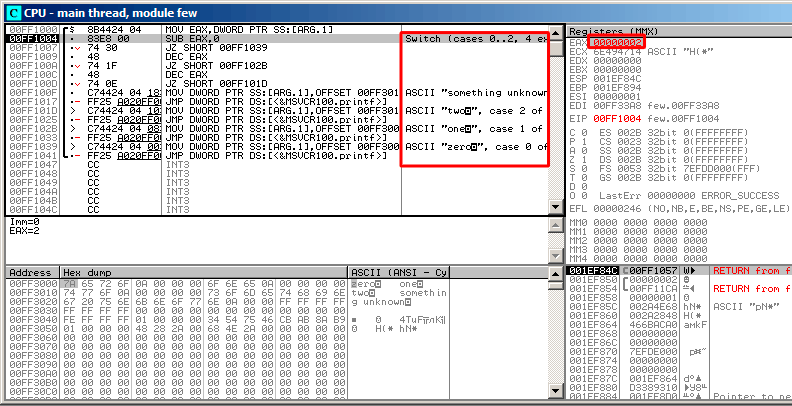
\includegraphics[scale=\FigScale]{patterns/08_switch/1_few/olly1.png}
\caption{\olly: \EAX \RU{содержит первый (и единственный) аргумент функции}
\EN{now contain the first (and only) function argument}}
\label{fig:switch_few_olly1}
\end{figure}

\clearpage
0 \RU{отнимается от}\EN{is subtracted from} 2 \InENRU \EAX. 
\RU{Конечно же}\EN{Of course}, \EAX \RU{всё ещё содержит}\EN{still contains} 2.
\RU{Но флаг}\EN{But the} \ZF \RU{теперь}\EN{flag is now} 0, \RU{что означает, что последнее вычисленное значение
не было нулевым}\EN{indicating that the resulting value is non-zero}:

\begin{figure}[H]
\centering
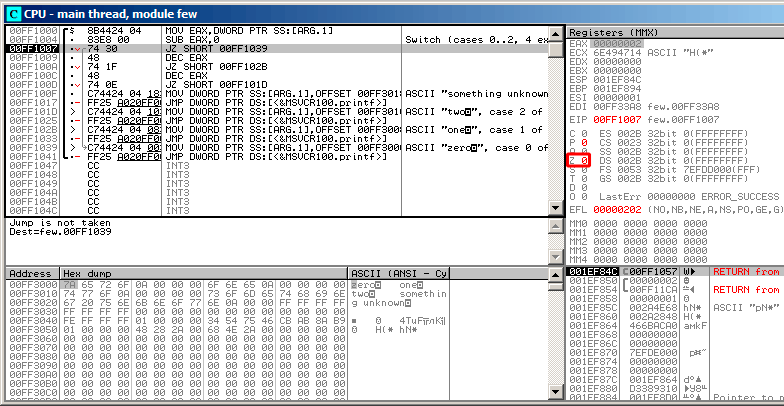
\includegraphics[scale=\FigScale]{patterns/08_switch/1_few/olly2.png}
\caption{\olly: \SUB \RU{исполнилась}\EN{executed}}
\label{fig:switch_few_olly2}
\end{figure}

\clearpage
\DEC \RU{исполнилась и}\EN{is executed and} \EAX \RU{теперь содержит}\EN{now contains} 1. 
\RU{Но}\EN{But} 1 \RU{не ноль, так что флаг}\EN{is non-zero, so the} \ZF \RU{всё ещё}\EN{flag is still} 0:

\begin{figure}[H]
\centering
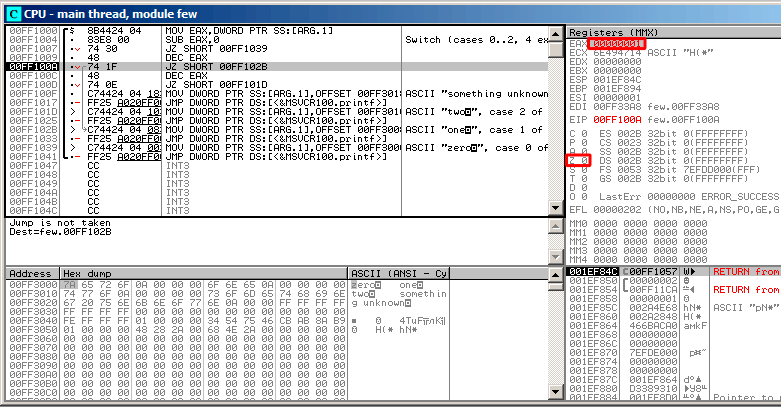
\includegraphics[scale=\FigScale]{patterns/08_switch/1_few/olly3.png}
\caption{\olly: \RU{первая}\EN{first} \DEC \RU{исполнилась}\EN{executed}}
\label{fig:switch_few_olly3}
\end{figure}

\clearpage
\RU{Следующая}\EN{Next} \DEC \RU{исполнилась}\EN{is executed}. 
\EAX \RU{наконец}\EN{is finally} 0 \RU{и флаг}\EN{and the} \ZF \RU{выставлен, потому что результат~--- ноль}\EN{flag
gets set, because the result is zero}:

\begin{figure}[H]
\centering
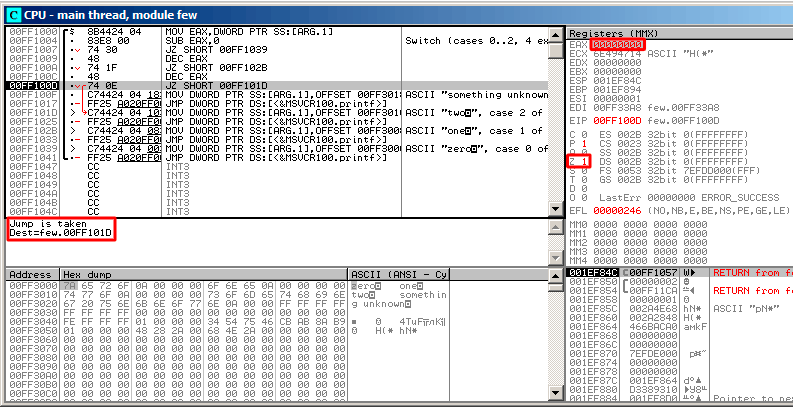
\includegraphics[scale=\FigScale]{patterns/08_switch/1_few/olly4.png}
\caption{\olly: \RU{вторая}\EN{second} \DEC \RU{исполнилась}\EN{executed}}
\label{fig:switch_few_olly4}
\end{figure}

\olly \RU{показывает, что условный переход сейчас сработает.}
\EN{shows that this jump is to be taken now.}

\clearpage
\RU{Указатель на строку}\EN{A pointer to the string} \q{two} 
\RU{сейчас будет записан в стек}%
\EN{is to be written into the stack now}:

\begin{figure}[H]
\centering
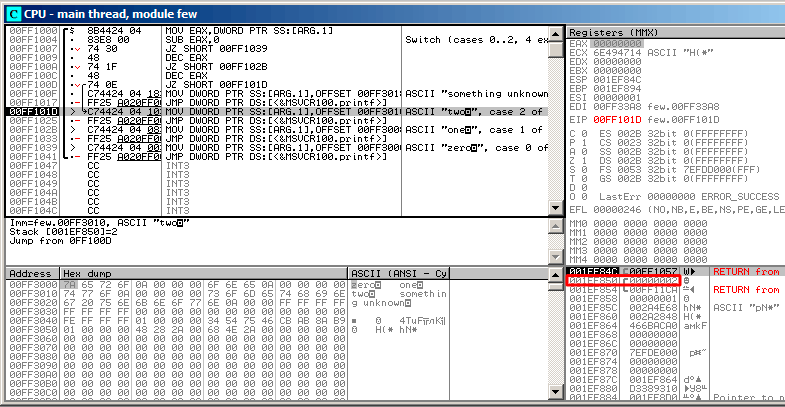
\includegraphics[scale=\FigScale]{patterns/08_switch/1_few/olly5.png}
\caption{\olly: \RU{указатель на строку сейчас запишется на место первого аргумента}
\EN{pointer to the string is to be written at the place of the first argument}}
\label{fig:switch_few_olly5}
\end{figure}

<<<<<<< HEAD
% TODO: homogenize numbers
% now they are inconsistent: sometimes plain text, sometimes in math mode
=======
>>>>>>> dbc594242ac84ce9f90c4cdb9027b16c0cfab328
\RU{Обратите внимание: текущий аргумент функции это 2 и 2 прямо сейчас в стеке по адресу}\EN{Please note: 
the current argument of the function is 2 and 2 is now in the stack at the address} \TT{0x0020FA44}.

\clearpage
\MOV \RU{записывает указатель на строку по адресу}\EN{writes the pointer to the string at address} 
\TT{0x0020FA44} (\RU{см. окно стека}\EN{see the stack window}).
\RU{Переход сработал}\EN{Then, jump happens}.
\RU{Это самая первая инструкция функции}\EN{This is the first instruction of the} \printf \RU{в}\EN{function in} 
MSVCR100.DLL (\RU{я скомпилировал этот пример с опцией /MD}\EN{I compiled the example with /MD switch}): 

\begin{figure}[H]
\centering
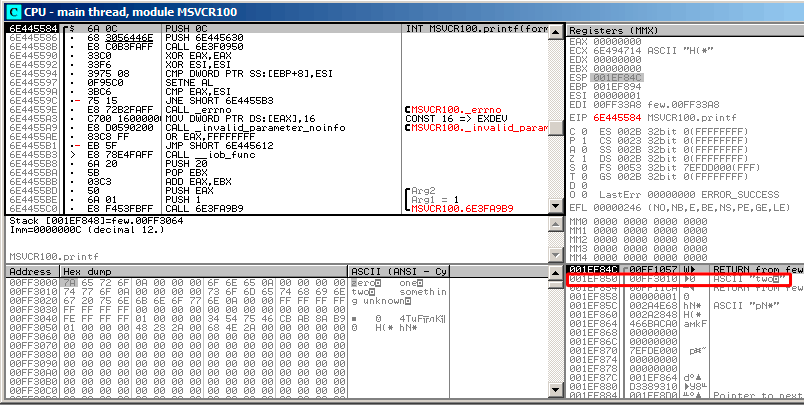
\includegraphics[scale=\FigScale]{patterns/08_switch/1_few/olly6.png}
\caption{\olly: \RU{первая инструкция в}\EN{first instruction of} \printf \InENRU MSVCR100.DLL}
\label{fig:switch_few_olly6}
\end{figure}

\RU{Теперь}\EN{Now} \printf \RU{считает строку на}\EN{treats the string at} \TT{0x00FF3010} 
\RU{как свой единственный аргумент и выводит строку}\EN{as its only argument and prints the string}.

\clearpage
\RU{Это самая последняя инструкция функции}\EN{This is the last instruction of} \printf:

\begin{figure}[H]
\centering
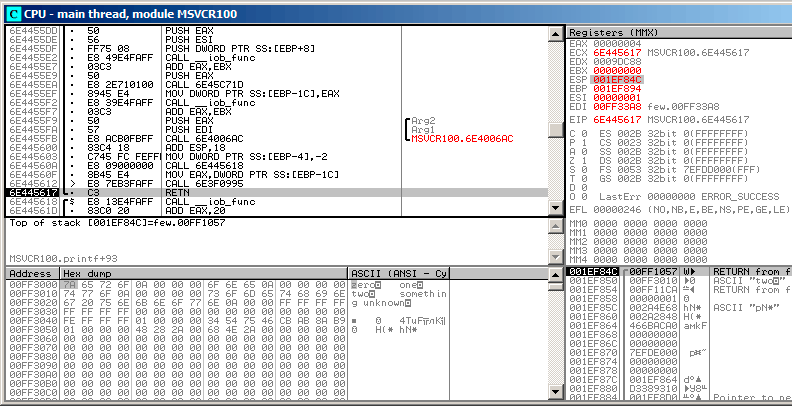
\includegraphics[scale=\FigScale]{patterns/08_switch/1_few/olly7.png}
\caption{\olly: \RU{последняя инструкция в}\EN{last instruction of} \printf \InENRU MSVCR100.DLL}
\label{fig:switch_few_olly7}
\end{figure}

\EN{The string}\RU{Строка} \q{two} \RU{была только что выведена в консоли}\EN{was just printed to the console window}.

\clearpage
\RU{Нажмем}\EN{Now let's press} F7 \OrENRU F8 (\stepover) \RU{и вернемся}\EN{and return}\dots
\RU{нет, не в функцию}\EN{not to} \ttf \RU{но в}\EN{, but rather to} \main:

\begin{figure}[H]
\centering
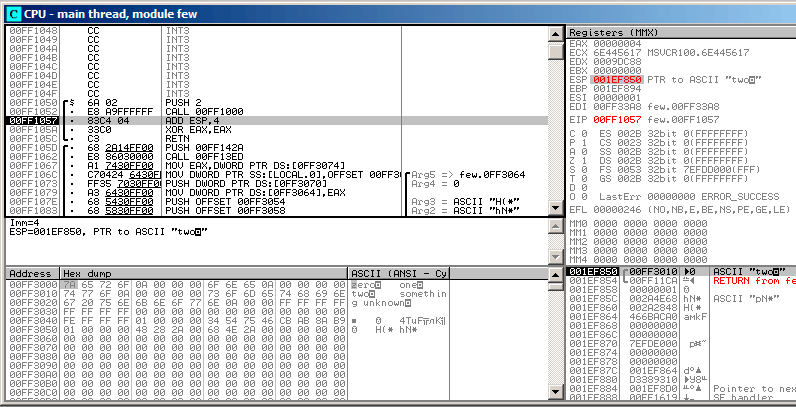
\includegraphics[scale=\FigScale]{patterns/08_switch/1_few/olly8.png}
\caption{\olly: \RU{возврат в}\EN{return to} \main}
\label{fig:switch_few_olly8}
\end{figure}

\RU{Да, это прямой переход из внутренностей}\EN{Yes, the jump was direct, from the guts of} \printf 
\RU{в}\EN{to} \main.
\RU{Потому как}\EN{Because} \ac{RA} \RU{в стеке указывает не на какое-то место в функции}\EN{in the stack points 
not to some place in} \ttf \RU{а в}\EN{, but rather to} \main.
\RU{И}\EN{And} \CALL \TT{0x00FF1000} \RU{это инструкция вызывающая функцию}\EN{was the actual instruction which called} 
\ttf.
